\documentclass{article}
\usepackage{style}

\usepackage[margin = 1.25in]{geometry}

\captionsetup{justification = centering}

\title{A Cosimplicial Object in the Category of Type Theories}
\author{Zack Dooley}
\date{}

\begin{document}
\maketitle

\section{A Nerve for Type Theories}

We start with a short introduction to globular sets, which will be necessary to defining composition of cells, or iterated identity types, within a type theory.

\begin{defn}
    A \textbf{globular set}, $G$ is a sequence of sets equipped with source and target functions $(G_n,s_n,t_n)_{n\in\N}$, where the functions $s_n,t_n\colon G_{n+1}\to G_n$ satisfy the following equations,
    $$ t_nt_{n+1}=t_ns_{n+1},\qquad s_ns_{n+1}=s_nt_{n+1}. $$
    We refer to elements of $G_n$ as $n$-\textbf{cells}.
\end{defn}

The relations on the source and target maps ensure that each $n$-cell $\alpha$ has a unique $m$-source/target for all $m<n$ given by $s_ms_{m+1}\cdots s_{n-1}\alpha$ and $t_mt_{m+1}\cdots t_{n-1}\alpha$ respectively, which we will just denote by $s_m\alpha$ and $t_m\alpha$ in the future.

\begin{defn}
    A \textbf{reflexive} globular set is a tuple $(G_n,s_n,t_n,i_n)_{n\in\N}$, such that $(G_n,s_n,t_n)_{n\in\N}$ is a globular set, and $\{i_n\colon G_n\to G_{n+1}\}_{n\in\N}$ is a sequence of maps such that $s_ni_n=\id=t_ni_n$.
\end{defn}

We think of these maps as giving reflexivity $(n+1)$-cells from a given $n$-cell.

Before we define the reflexive globular set that we will be working with, we establish some notation for iterated identity types originally due to \cite{AHW}.

\begin{notn}
    If $A$ is a type, then we define $\Id_A^0:=A$ and if $a,b:A$, then $\Id_A^1(a,b):=\Id_A(a,b)$. Now, given $a_{n+1},b_{n+1}:\Id_A^n(a_1,b_1;\dots;a_n,b_n)$, we inductively define
    $$ \Id_A^{n+1}(a_1,b_1;\dots;a_n,b_n;a_{n+1},b_{n+1}):=\Id_{\Id^n_A(a_1,b_1;\dots;a_n,b_n)}(a_{n+1},b_{n+1}). $$
\end{notn}

With this, we can define the reflexive globular set $\Gamma(\T,S)$ of a set of closed types $S$ in some type theory $\T$\footnote{This construction is an adaptation of a similar construction designed for a single type found in \cite{AHW}.}. For simplicity, we will define $\Gamma(\T):=\Gamma(\T,\{\text{all closed types of }\T\})$.

\begin{defn}
    Let
    $$ \Gamma(\T,S)_0:=S, $$
    $$ \Gamma(\T,S)_1=\left\{(A_0,A_1;\gamma)\ |\ A_i\in\Gamma(\T,S)_0\text{ and }x:A_0\vdash\gamma(x):\Id^0_{A_1}\right\}, $$
    with $s_1,t_1$ being the first and second projections respectively. From here, we define the remaining levels inductively (We omit the dependency of $\gamma(x)$ on $x$ when it is clear). For $n>1$, we define
    $$ \Gamma(\T,S)_{n+1}:=\left\{(A_0,A_1;\vec{\alpha};\beta_0,\beta_1;\gamma)\ |\ (A_0,A_1;\vec{\alpha};\beta_i)\in\Gamma(\T,S)_n\text{ and }x:A_0\vdash\gamma(x):\Id_{A_1}^{n}(\vec{\alpha};\beta_0(x),\beta_1(x))\right\}, $$
    with $s_{n+1},t_{n+1}$ given by $(A_0,A_1;\vec{\alpha};\beta_0,\beta_1;\gamma)\mapsto(A_0,A_1;\vec{\alpha};\beta_i)$ with $i=0,1$ respectively. Reflexivity at level 0 is given by the map $i_0:\Gamma(\T,S)_0\to\Gamma(\T,S)_1$ which sends $A$ to  $(A,A;x:A\vdash x:A)$. Above level 0, reflexivity is given by the maps $i_n:\Gamma(\T,S)_n\to\Gamma(\T,S)_{n+1}$ which sends $(\vec{\alpha};\beta)$ to $(\vec{\alpha};\beta,\beta;\refl_{\beta(x)})$. The relevant identities are easily verified.
\end{defn}

We now wish to define composition operations on $\Gamma(\T,S)$ for all $m\in\N$, giving it the structure of a sort of (weak) infinity category. To define composition, we first define when two cells are composable.

\begin{defn}
    We say two $n$-cells $\alpha,\alpha'\in\Gamma(\T,S)_n$ are $m$-\textbf{composable} when $s_m(\alpha)=t_m(\alpha')$.
\end{defn}

Note that being $m$-composable implies that $m<n$. We can now define $m$-composition on $m$-composable $n$-cells by induction on $n$.

\begin{defn}
    For $n=1$, we define
    $$ (A_0,A_1;\gamma(y))\circ_0(A_0',A_1';\gamma'(x)):=(A_0',A_1;\gamma(\gamma'(x))), $$
    noting that $A_0=A_1'$ because our cells are 0-composable. Now assuming we can $m$-compose $n$-cells for all $m<n$, we define $m$-composition of $(n+1)$-cells,
    $$ (A_0,A_1;\vec{\alpha};\beta_0,\beta_1;\gamma)\circ_m(A'_0,A'_1;\vec{\alpha}';\beta_0',\beta_1';\gamma') $$
    with two cases. First, if $m=n$, then our inductive hypothesis cannot help us, so we instead just apply path concatenation (which path concatenation?), which applies as $(A_0,A_1;\vec{\alpha};\beta_0,\beta_1;\gamma)$ and $(A'_0,A'_1;\vec{\alpha}';\beta_0',\beta_1';\gamma')$ are $n$-composable, so we get
    $$ (A_0,A_1;\vec{\alpha};\beta_0,\beta_1;\gamma)\circ_n(A'_0,A'_1;\vec{\alpha}';\beta_0',\beta_1';\gamma'):=(A_0,A_1;\vec{\alpha};\beta_0',\beta_1;\gamma*\gamma'). $$
    If $m<n$, then we apply path induction to both $\gamma$ and $\gamma'$ to reduce the problem to
    \begin{align*}
        (A_0,A_1;\vec{\alpha};\beta_0(x),\beta_0(x);\refl_{\beta_0(x)})&\circ_m(A'_0,A'_1;\vec{\alpha}';\beta_0'(x),\beta_0'(x);\refl_{\beta_0'(x)})\\
        &=i_{n+1}(A_0,A_1;\vec{\alpha};\beta_0(x))\circ_mi_{n+1}(A'_0,A'_1;\vec{\alpha}';\beta_0'(x))\\
        &:=i_{n+1}\left((A_0,A_1;\vec{\alpha};\beta_0(x))\circ_m(A'_0,A'_1;\vec{\alpha}';\beta_0'(x))\right).
    \end{align*}
\end{defn}

We note that the final composition is well defined by our inductive hypothesis, since $(A_0,A_1;\vec{\alpha};\beta_0,\beta_1;\gamma)$ and $(A'_0,A'_1;\vec{\alpha}';\beta_0',\beta_1';\gamma')$ being $m$-composable, implies $(A_0,A_1;\vec{\alpha};\beta_0)$ and $(A'_0,A'_1;\vec{\alpha}';\beta_0')$ are $m$-composable as well.

To be completely formal, we note that the composition $(A,B;\vec{\alpha};a_n,b_n;\gamma)\circ_m(A',B';\vec{\alpha}';a'_n,b'_n;\gamma')$, explicitly relies on a composition defined on iterated identity types, i.e. given judgments of the form
$$ x:A_0\vdash\gamma(x):\Id_{A_1}^n(\vec{\alpha};a_m,b_m;a_{m+1},b_{m+1};\dots;a_n,b_n) $$
$$ x:A_0\vdash\gamma'(x):\Id_{A_1}^n(\vec{\alpha};a'_m,a_m;a'_{m+1},b'_{m+1};\dots;a'_n,b'_n) $$
We wish to construct a term of type
$$ x:A_0\vdash\Id_{A_1}^n(\vec{\alpha};a'_m,b_m;a_{m+1}\circ_ma'_{m+1},b_{m+1}\circ_mb'_{m+1};\dots;a_n\circ_ma'_n,b_n\circ_mb'_n)\text{ Type}, $$
Which is well defined by the inductive hypotheses. We construct this term by path induction on $\gamma$ and $\gamma'$ as stated above, denoting the resulting term $\gamma\circ_m\gamma'$. This shows us that $\circ_m$ is not just an operation on $\Gamma(\T,S)$, but on the underlying (iterated) identity types as well.

Note then that with this we can define the $m$-composition of an $n$-cell $\gamma$ with an $\ell$-cell $\delta$ ($m<\ell<n$),
$$ x:A_0\vdash\gamma(x):\Id_{A_1}^{n-1}(\vec{\alpha};a_m,b_m;a_{m+1},b_{m+1};\dots;a_{n-1},b_{n-1}) $$
$$ x:A_0\vdash\delta(x):\Id_{A_1}^{\ell-1}(\vec{\alpha};a'_m,a_m;a'_{m+1},b'_{m+1};\dots;a'_{\ell-1},b'_{\ell-1}), $$
as a term of type
$$ x:A_0\vdash\Id_{A_1}^{n-1}(\vec{\alpha};a'_m,b_m;a_{m+1}\circ_ma'_{m+1},b_{m+1}\circ_mb'_{m+1};\dots;a_\ell\circ_m\delta,b_\ell\circ_m\delta;\dots;a_{n-1}\circ_m\delta,b_n\circ_m\delta)\text{ Type}, $$
given by path induction on $\gamma$, which allows us to inhabit the previous type with $\refl_{a_n\circ_m\delta}$.
% Clean up definition, do comp on id types first
% need to do induction on both cells, 0 composition of 0-cells is different depending on direction

We wish to show that this composition has (weak) group-like properties. To do so we define $m$-inverses of $n$-cells, where $m<n$.

\begin{defn}
    We proceed by induction on $n$. Let $n=2$ and $\gamma=(A,B;a_1,b_1;\gamma)$ be a 2-cell (note we are conflating the element of $\Gamma(\T,S)_2$ with its final projection). We define $\bar{\gamma}_{(1)}:=(A,B,b_1,a_1,\bar{\gamma})$, where $\bar{\gamma}$ is our standard notion of an inverse path in an identity type.

    Assuming now that we have constructed $m$-inverses of $n$-cells (with $1\leq m<n$ and $n\geq2$), if $\gamma=(A,B;\vec{\alpha};a_n,b_n;\gamma)$ in an $n$-cell, then we define $\bar{\gamma}_{(m)}$ with two cases. If $m=n$, then $\bar{\gamma}_{(n)}:=\bar{\gamma}$, the usual inverse path as before. Otherwise, to define $\bar{\gamma}_{(m)}$, we wish to construct a term of the type
    $$ \Id_A^n(\vec{\alpha}_{<m};b_{m},a_m;\bar{a}_{m+1,(m)},\bar{b}_{m+1,(m)};\dots;\bar{a}_{n,(m)},\bar{b}_{n,(m)}), $$
    which is well defined by our inductive hypothesis. To construct this term, we apply path induction to $\gamma$, resulting in the type above changing to
    $$ \Id_A^n(\vec{\alpha}_{<m};b_{m},a_m;\bar{a}_{m+1,(m)},\bar{b}_{m+1,(m)};\dots;\bar{a}_{n,(m)},\bar{a}_{n,(m)}), $$
    which is inhabited by the term $\refl_{\bar{a}_{n,(m)}}$, so path induction gives us our desired term $\bar{\gamma}_{(m)}$. % This could probably be written a little clearer/better notation maybe
\end{defn}

We will now prove the proper identity, inverse, and associativity laws for this composition, but first we establish a bit of notation.

\begin{notn}
    If $a:A$, then we denote the iterated reflexivity term on $a$ as follows,
    $$ \refl^n_a:=\overbrace{\refl_{\ddots_{\refl_a}}}^{n\text{ times}}:\Id^{n-1}_A\left(a,a;\refl_a,\refl_a;\dots;\overbrace{\refl_{\ddots_{\refl_a}}}^{(n-1)\text{ times}},\refl_{\ddots_{\refl_a}}\right). $$
    We take $\refl^0_a:=a$.
\end{notn}

\begin{prop}\label{prop:unit}
    For an $n$-cell $\gamma$, and any $0<m<n$, we have
    $$ \tr^{2((n-1)-m)}(\gamma\circ_m\refl^{n-m}_{a_m})=\gamma=\tr^{2((n-1)-m)}(\refl^{n-m}_{b_m}\circ_m\gamma). $$
\end{prop}
\begin{proof}
    We prove this by induction on $n$. For $n=2$, we have that $\gamma\circ_1\refl_{a_1}$ is defined by regular path concatenation, so the statement reduces to a standard fact about identity types, proven by path induction on $\gamma$.

    Now assuming that $\tr^{2((n-1)-m)}(\gamma\circ_m\refl^{n-m}_{a_m})=\gamma$ for all cells below level $n$, where the term $\tr^{2((n-1)-m)}(\gamma\circ_m\refl^{n-m}_{a_m})$ is itself defined inductively by transporting over each path $\tr^{2((i-1)-m)}(\gamma\circ_m\refl^{i-m}_{a_m})=\gamma$ for $m<i<n$, so that if
    $$ \gamma\circ_m\refl^{n-m}_{a_m}:\Id_B^{n-1}\left(\vec{\alpha};a_m,b_m;a_{m+1}\circ_m\refl_{a_m},b_{m+1}\circ_m\refl_{a_m};\dots;a_{n-1}\circ_m\refl_{a_m}^{(n-1)-m},b_{n-1}\circ_m\refl_{a_m}^{(n-1)-m}\right), $$
    then
    $$ \tr^{2((n-1)-m)}(\gamma\circ_m\refl^{n-m}_{a_m}):\Id_B^{n-1}\left(\vec{\alpha};a_m,b_m;a_{m+1},b_{m+1};\dots;a_{n-1},b_{n-1}\right), $$
    noting that all involved paths were on $(n-1)$-cells and below (the factor of two comes from having to transport over both the source and target at every level). If $\gamma$ is an $n$-cell then to show $\tr^{2((n-1)-m)}(\gamma\circ_m\refl^{n-m}_{a_m})=\gamma$, we apply path induction to $\gamma$, reducing the problem to $\tr^{2((n-1)-m)}(\refl_{a_n}\circ_m\refl^{n-m}_{a_m})=\refl_{a_n}$. If we now apply repeated path induction to the $a_i's$ in the left hand side of the composition, we can reduce this to $\tr^{2((n-1)-m)}(\refl^{n-m}_{a_m}\circ_m\refl^{n-m}_{a_m})=\refl^{n-m}_{a_m}$. Now by the definition of composition, we get that $\refl^{n-m}_{a_m}\circ_m\refl^{n-m}_{a_m}$ is definitionally equal to $\refl^{n-m}_{a_m}$, so all the transports are now occurring along reflexivity paths, and thus acting as the identity, so to complete the path induction, we just need a term of type $\refl^{n-m}_{a_m}=\refl^{n-m}_{a_m}$, which is given by reflexivity.

    The proof of $\gamma=\tr^{2((n-1)-m)}(\refl^{n-m}_{b_m}\circ_m\gamma)$ is symmetric except that it requires applying path induction in the second argument on $\gamma$. % is this allowed?
\end{proof}

\begin{prop}\label{prop:inverse}
    For an $n$-cell $\gamma$, and any $0<m<n$, we have
    $$ \tr^{2((n-1)-m)}(\gamma\circ_m\bar{\gamma}_{(m)})=\refl^{n-m}_{b_m}\quad\text{and}\quad\tr^{2((n-1)-m)}(\bar{\gamma}_{(m)}\circ_m\gamma)=\refl^{n-m}_{a_m}. $$
\end{prop}
\begin{proof}
    We prove this by induction on $n$. For $n=2$, we get that $\gamma\circ_m\bar{\gamma}_{(m)}:=\gamma*\bar{\gamma}$, which we know is (prepositionally) equal to $\refl_{b_1}$ by standard arguments.

    For the inductive step, we assume that $\tr^{2((n-1)-m)}(\gamma\circ_m\bar{\gamma}_{(m)})=\refl^{n-m}_{b_m}$ is true for all cells below level $n$ and all $0<m<n$, and as in the previous proof, we inductively define the following term for a given $n$-cell $\gamma$,
    $$ \tr^{2((n-1)-m)}(\gamma\circ_m\bar{\gamma}_{(m)}):\Id_B^{n-1}(\vec{\alpha};b_m,b_m;\refl_{b_m},\refl_{b_m};\dots;\refl^{n-1-m}_{b_m},\refl^{n-1-m}_{b_m}), $$
    by transporting over the equalities given by our inductive hypothesis. To get the desire equality then, we just apply repeated path induction to $\gamma$, reducing $\tr^{2((n-1)-m)}(\gamma\circ_m\bar{\gamma}_{(m)})$ to $\tr^{2((n-1)-m)}(\refl^{n-m}_{b_m}\circ_m\overline{\refl^{n-m}_{b_m}}_{(m)})$. Noting that $\overline{\refl^{n-m}_{b_m}}_{(m)}$ is definitionally equal to $\refl^{n-m}_{b_m}$ and the composition of reflexivity is reflexivity, this reduces us to finding a term of the type $\refl^{n-m}_{b_m}=\refl^{n-m}_{b_m}$ (since we're reduced to transporting over reflexivity), which is given by reflexivity. The proof of $\tr^{2((n-1)-m)}(\bar{\gamma}_{(m)}\circ_m\gamma)=\refl^{n-m}_{a_m}$ is analogous.
\end{proof}

\begin{prop}\label{prop:assoc}
    For $n$-cells $\gamma,\delta,\beta$, and any $0<m<n$, we have
    $$ \tr^{(n-1)-m}((\beta\circ_r\delta)\circ_r\gamma)=\beta\circ_r(\delta\circ_r\gamma). $$
\end{prop}
\begin{proof}
    This proof follows similarly to the previous two. We prove this by induction on $n$. In the base case, the problem is reduced to traditional associativity of path composition. For the inductive step, we use the inductive hypothesis to define the term $\tr^{(n-1)-m}(\beta\circ_r(\delta\circ_r\gamma))$, and we apply repeated path induction to $\gamma,\delta$, and $\beta$. Since the composition of reflexivity terms is definitionally reflexivity, this reduces the problem to finding a term of type $\refl^{n-m}_{a_m}=\refl^{n-m}_{a_m}$, which is given by reflexivity.
\end{proof}

With this, we wish to start to defining our cosimplicial object in the category of type theories (by this we mean $\CxlCat_{\Id}$, the category of contextual categories with $\Id$ type structures) by defining the type theories, $\bS_n$ for each $n\in\N$. Fundamental to this construction is translating between the globular structure of types/type theories, and simplicial structures. To do so, we use a combinatorial solution from \cite{Street}, which is used to construct a nerve functor for strict $\omega$-categories. Since our construction relies heavily on the results in that paper, we review some of the relevant information.

\begin{defn}
    A \textbf{category} $(A,s,t,*)$ consists of a set $A$, functions $s,t\colon A\to A$ satisfying 
    $$ ss=ts=s,\qquad tt=st=t, $$
    and a function $*:\{(a,b)\in A\times A\ |\ s(a)=t(b)\}\to A$ satisfying
    $$ s(a*b)=s(b),\qquad t(a*b)=t(a), $$
    such that the following axioms hold:
    \begin{align*}
        &s(a)=t(v)=v\quad\text{implies}\quad a*v=a,\\
        &u=s(u)=t(a)\quad\text{implies}\quad u*a=a,\\
        &a*(b*c)=(a*b)*c.
    \end{align*}
\end{defn}

\begin{defn}
    A \textbf{2-category} $(A,s_0,t_0,*_0,s_1,t_1,*_1)$ consists of two categories $(A,s_i,t_i,*_i)$ ($i\in\{0,1\}$) satisfying the following equations:
    \begin{enumerate}
        \item $s_1s_0=s_0=s_0s_1=s_0s_1=s_0t_1,\quad t_0=t_0s_1=t_0t_1,$
        \item $s_1(a*_0b)=s_1(a)*_0s_1(b),\quad t_1(a*_0b)=t_1(a)*_0t_1(b),$
        \item $(a*_1 b)*_0(a'*_1b')=(a*_0a')*_1(b*_0b').$
    \end{enumerate}
\end{defn}

\begin{defn}
    A (strict) $\omega$-\textbf{category} $(A,(s_n,t_n,*_n)_{n\in\N})$ consists of categories $(A,s_n,t_n,*_n)$ for all $n\in\N$, such that $(A,s_m,t_m,*_m,s_n,t_n*_n)$ is a 2-category for all $m<n$.
\end{defn}

We refer to the identities of the operations $*_n$ as $n$-\textbf{cells}. Note that this definition is very similar to that of a globular set (with composition operations), except our $\omega$-categories are single-sorted, with just a single set $A$, as opposed to our globular sets which are $\N$-graded. We use this non-standard definition of $\omega$-categories to match the exposition given in \cite{Street}.

Now to construct the cosimplicial object in $\omega$-categories, Street defines the oriented simplicies $\cO_n$ for each $n\in\N$ in a few steps, starting with the $\omega$-category $\cN$.

\begin{defn}
    Let $\cN$ be an $\omega$-category whose elements are double sequences $a=(a_n^1,a_n^0)_{n\in\N}$, where $a_n^p$ is a finite subset of $\binom{\N}{n+1}$, the set of size $n+1$ subsets of $\N$. Source and target maps are given by the following formulas:
    $$ s_n(a)^q_m=\begin{cases}
        a_m^q & \text{for }m<n,\\
        a_n^1 & \text{for }m=n,\\
        \emptyset & \text{for }m>n;
    \end{cases}\qquad
    t_n(a)^q_m=\begin{cases}
        a_m^q & \text{for }m<n,\\
        a_n^0 & \text{for }m=n,\\
        \emptyset & \text{for }m>n.
    \end{cases} $$
    For $s_n(a)=t_n(b)$, the composite $a*_nb$ is given by the formula:
    $$ (a*_nb)_m^q=\begin{cases}
        a_m^q=a_m^q & \text{for }m<n,\\
        b_n^1 & \text{for }q=1\text{ and }m=n,\\
        a_n^0 & \text{for }q=0\text{ and }m=n,\\
        a_m^q\cup b_m^q & \text{for }m>n.
    \end{cases} $$
\end{defn}

To define the subcategory $\cO_\omega$ of $\cN$, which we will obtain our oriented simplicies from, we first need to define a property of subsets of $\binom\N{m+1}$. First, we note that subsets of $\N$ come with a natural ordering, so thinking of them as simplices, we can define face maps $\partial_i\colon{\binom\N m+1}\to{\binom\N m}$ for all $m\in\N$ and $i\leq m+1$, which remove the $i$-th element.

\begin{defn}
    We call a subset $S\subseteq{\binom\N{m+1}}$ \textbf{well-formed} when distinct elements of $S$ have no faces of the same parity, i.e. if $x,y\in S$ and $x\partial_i=y\partial_j$ for some $i,j$ of the same parity, then $x=y$.
\end{defn}

We also define the even and odd faces of a set $S\subseteq{\binom\N{m+1}}$ by
$$ \phi^pS:=\{x\partial_i\ |\ x\in S,\ i\text{ of same parity as }p\}. $$
With this we can introduce some notation for the set of even faces which are not odd (and vice versa),
$$ \rho^1S:=\phi^1S\setminus\phi^0S\quad\text{and}\quad\rho^0S:=\phi^0S\setminus\phi^1S. $$
With this we can now give the definition of Street's oriented simplicies.

\begin{defn}
    The $\omega$-category $\cO_\omega$ is defined as the subcategory of $\cN$ consisting of all elements $a\in\cN$ such that for all $p,q\in\{0,1\}$ and $m\in\N$:
    \begin{enumerate}
        \item $a_m^p$ is well formed,
        \item $a_m^p=\rho^pa_{m+1}^q\sqcup (a_m^0\cap a_m^1)$.
    \end{enumerate}
\end{defn}

While it is easy to see that the source and target functions restrict to $\cO_\omega$, it is not at all clear that the composition functions do, but proving this is an evolved process, so for that we refer to \cite{Street}. To get the actual oriented simplicies $\cO_n$, we can now just restrict $\cO_\omega$ to all elements $a$ such that $a_m^p\subseteq{\binom{[n]}{m+1}}$ for all $p\in\{0,1\}$ and $m\in\N$.

For our purposes, we will also like to define a filtration on $\cO_n$ given by removing elements of higher dimensions.

\begin{defn}
    We define the $i$-\textbf{th truncation of the} $n$-\textbf{th oriented simplex} to be
    $$ \cO_{n,i}:=\{b\in\cO_n\ |\ b^p_m=\emptyset\text{ for }m>i\}. $$
\end{defn}

These definition can appear somewhat opaque, but they do result in the geometric interpretations that we desire i.e. unwinding all the combinatorics, we can see that each $\cO_n$ is freely generated by a set of cells, $\gen{z}$ for $z\subseteq[n]$, which have our desired geometric semantics, as seen in the following diagrams.
\begin{figure}[htp]
\[\begin{tabular}{wc{2cm}>{\centering\arraybackslash}m{10cm}}
    $\cO_0$ & $\gen{0}$\\
    \\
    $\cO_1$ & 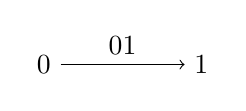
\begin{tikzpicture}
        \node (0) at (0,0) {$\gen{0}$};
        \node (1) at (2,0) {$\gen{1}$};
        \draw[->] (0) to node[above]{$\gen{01}$} (1);
    \end{tikzpicture}\\
    \\
    $\cO_2$ &  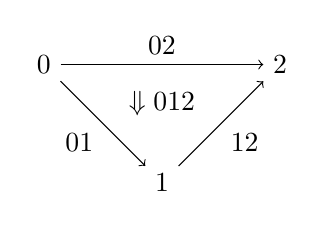
\begin{tikzpicture}
        \node (0) at (0,0) {$\gen{0}$};
        \node (1) at (1.5,-1.5) {$\gen{1}$};
        \node (2) at (3,0) {$\gen{2}$};
        \node (012) at (1.5,-0.5) {$\Downarrow\gen{012}$};
        \draw[->] (0) to node[below left]{$\gen{01}$} (1);
        \draw[->] (0) to node[above]{$\gen{02}$} (2);
        \draw[->] (1) to node[below right]{$\gen{12}$} (2);
    \end{tikzpicture}\\
    \\
    $\cO_3$ & 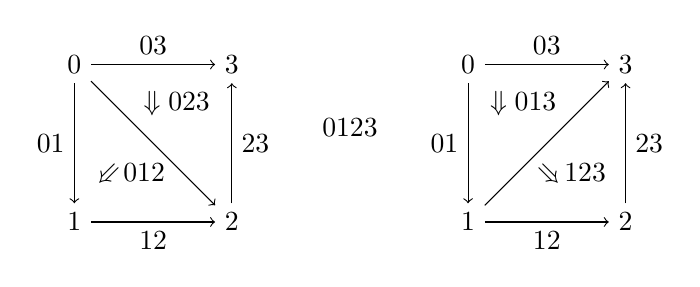
\begin{tikzpicture}
        \node (0) at (0,0) {$\gen{0}$};
        \node (1) at (0,-2) {$\gen{1}$};
        \node (2) at (2,-2) {$\gen{2}$};
        \node (3) at (2,0) {$\gen{3}$};
        \node (023) at (1.3,-0.5) {$\Downarrow\gen{023}$};
        \node (012) at (0.7,-1.4) {$\mathbin{\rotatebox[origin=c]{-45}{$\Downarrow$}}\gen{012}$};
        \draw[->] (0) to node[above]{$\gen{03}$} (3);
        \draw[->] (0) to node[left]{$\gen{01}$} (1);
        \draw[->] (0) to (2);
        \draw[->] (1) to node[below]{$\gen{12}$} (2);
        \draw[->] (2) to node[right]{$\gen{23}$} (3);

        \node (0123) at (3.5,-0.8) {$\gen{0123}$};
        \node (A) at (3.5,-1.2) {$\Rrightarrow$};

        \node (0') at (5,0) {$\gen{0}$};
        \node (1') at (5,-2) {$\gen{1}$};
        \node (2') at (7,-2) {$\gen{2}$};
        \node (3') at (7,0) {$\gen{3}$};
        \node (013) at (5.7,-0.5) {$\Downarrow\gen{013}$};
        \node (123) at (6.3,-1.4) {$\mathbin{\rotatebox[origin=c]{45}{$\Downarrow$}}\gen{123}$};
        \draw[->] (0') to node[above]{$\gen{03}$} (3');
        \draw[->] (0') to node[left]{$\gen{01}$} (1');
        \draw[->] (1') to (3');
        \draw[->] (1') to node[below]{$\gen{12}$} (2');
        \draw[->] (2') to node[right]{$\gen{23}$} (3');
    \end{tikzpicture}
\end{tabular}\]
\caption{Diagrams of $\cO_n$ for $n=0,1,2,3$.}
\label{fig:diagrams}
\end{figure}

And so forth for for larger $n$ (diagrams of $\cO_4,\cO_5$, and $\cO_6$ can be found in \cite{Street}). To create type theories that act like these oriented simplices, we need an interpretation for these generating cells, but we already know what that is: closed types for the 0-cells, functions for the 1-cells, and identities for the higher cells. However, this introduces the primary problem, as to define these identity types, we need to know their endpoints, which will be given by complicated compositions of lower level cells. (more...) (Introduction)

Each $\cO_n$ is freely generated (in the sense of \cite[\S 4]{Street}) by more basic cells, each generated by a subset of $[n]$.

\begin{defn}
    Given a subset $z\subseteq[n]$, we define the term $\gen{z}$ by,
    $$ \gen{z}_m^p=\left\{x\in{\binom z{m+1}}\ |\ \text{if }r\in z\setminus x\text{ then }\#\{k\in x\ |\ k\leq r\}\text{ has parity }p\right\} $$
    for $p\in\{0,1\}$ and $m\in\N$.
\end{defn}

\begin{ex}
    Taking $z=[3]$, the formula above gives us the following 3-cell:
    $$ \gen{[3]}=\begin{pmatrix}
        \{\{3\}\}, & \{\{0,1\},\{1,2\},\{2,3\}\}, & \{\{1,2,3\},\{0,1,3\}\}, & \{[3]\}, & \emptyset, & \dots\\
        \{\{0\}\}, & \{\{0,3\}\}, & \{\{0,2,3\},\{0,1,2\}\}, & \{[3]\}, & \emptyset, & \dots\\
    \end{pmatrix}. $$
    Here the first row corresponds to $p=0$ and the second to $p=1$. Notice how the term $\gen{[3]}_m^0$ corresponds to what we might expect the $m$-target of the 3-cell in the 3-simplex to be, considering it globularly (similarly for $p=1$ and $m$-sources). For example, we can see that that two 2-cells that are in the source of the arrow $\gen{0123}$ in figure~\ref{fig:diagrams} are exactly the elements of $\gen{[3]}_2^1$. What this construction doesn't tells us, however, is how to compose those 2-cells in a way that type checks.
\end{ex}

% include some decompositions of relevent source/targets, corollary about full decomposition?

For the proofs that these $\gen{z}$ are in $\cO_\omega$ and that they freely generate it, again see \cite{Street}. These basic cells with be central to defining our interpretation function which makes use of the following theorem.

\begin{thm}[{\cite[Cor. 3.14]{Street}}]\label{thm:decomp}
    If $a\in\cO_\omega$ is an $n$-cell and $u\in a_n^1=a_n^0$ yet $a\neq\gen{u}$, then there exists $r\in[n-1]$ with $a=b*_r c$ for some $b,c\in\cO_\omega$ which are not $r$-cells.
\end{thm}

We note a slight modification to the proof of this theorem from \cite{Street} which will be necessary for our purposes. When choosing an element $w\in a_{r+1}^0\cap a_{r+1}^1$ which is then used to help define $a$ and $b$, we always choose the largest(?) such element, so that there are no choices made in this decomposition.

With this, we can finally start defining our type theories. We will build up $\bS_n$ inductively using intermediary type theories $\bS_n^{(i)}$ for $0\leq i\leq n$ ($\bS_n^{(n)}=\bS_n$), adding a new "dimension" of "cells" as generators for each layer. Simultaneously, we will define an interpretation function that will allow us to use combinatorics from \cite{Street}.

We start with our base type theory.

\begin{defn}
    Given $n\in\N$, we define our base type theory $\bS_n^{(0)}$ to be the type theory freely generated by closed types $A_j$ for all $j\in[n]$.
\end{defn}

Here we are considering our type theories to be contextual categories, so since the theory of contextual categories is essentially algebraic, we have a standard notion of what it mean to freely generate a contextual category.

We can now define the base case of our interpretation function, whose domain is defined as a subset of the $n$-th oriented simplex.

\begin{defn}
    Given $n\in\N$, we define a function
    $$ |-|_0\colon\mathcal{O}_{n,0}\to\bigsqcup_{m\in\N}\Gamma\left(\bS_n^{(0)}\right)_m $$
    by sending $\gen{b}\in\mathcal{O}_{n,0}$ to the element $A_{b}\in\Gamma\left(\bS_n^{(0)}\right)_0$.
\end{defn}

Here we note that by the definition of $\cO_{n,0}$, every element is of the form $\gen{b}$, where $b\subseteq[n]$ and $\#b=1$.

We can now simultaneously extend our base interpretation function and type theory inductively, assuming we have constructed the type theory $\bS_n^{(i)}$ and the interpretation function $|-|_i\colon\mathcal{O}_{n,i}\to\bigsqcup_{m\in\N}\Gamma\left(\bS_n^{(i)}\right)_m$.

\begin{defn}
    Given $n\in\N$, we define the type theory $\bS_n^{(i+1)}$ to be the type theory freely generated by the generators of $\bS_n^{(i)}$ along with terms
    $$ x:A_{\min(z)}\vdash a_z(x):\Id^{i-1}_{A_{\max(z)}}\left(|s_j(\gen{z})|_j,|t_j(\gen{z})|_j\right)\qquad(1\leq j\leq i), $$
    for all $z\subseteq[n]$ such that $\#z=i+1$.
\end{defn}

Note that by $|s_j(\gen{z})|_j,|t_j(\gen{z})|_j$, we really mean the final projection of this element-which is a term of the correct type and is dependent on $x$-as opposed to an element of $\Gamma(\bS_n^{(j)})$.

We now finish our inductive definition by extending our interpretation function.

\begin{defn}
    Given $n\in\N$, we define a function
    $$ |-|_{i+1}\colon\mathcal{O}_{n,i+1}\to\bigsqcup_{m\in\N}\Gamma\left(\bS_n^{(i+1)}\right)_m $$
    by sending $b\in\mathcal{O}_{n,i+1}$ to $|b|_i$ if $b\in\mathcal{O}_{n,i}$, or $\alpha_{b_1}=\left(|s_j(\gen{b_1})|_j,|t_j(\gen{b_1})|_j,a_{b_1}(x)\right)$ if $b=\gen{b_1}$ for some $b_1\subseteq[n]$. Otherwise, we apply Cor. 3.14 to get $b=b_1*_{k}b_2$ and we send this element to $|b_1|_{i+1}\circ_{k}|b_2|_{i+1}$.
\end{defn}
% 3.14 only works on n-cells, but everything in \mathcal{O}_{n,i+1} is an n-cell?

To make sure that this function is well-defined, we must have a consistent way of forming the decomposition given by Cor. 3.14, but this can be achieved by being consistent in our application of the corollary i.e. always decomposing the left most applicable element first, and being consistent in our choice of the element $w$ as described above. We also need to know that the process of applying the corollary repeatedly will terminate, but this is shown in \cite{Street}. Additionally, since $b^p_m=\emptyset$ for $m>i$, we know each of the $\gen{b_i}$ must be $i$-cells, so each $\alpha_{b_i}$ is an element of $\Gamma\left(\bS_n^{(i)}\right)_i$ (Noting that we are considering $A_{\max(b_i)}$ as a type in $\bS_n^{(i)}$ for the purpose of generating the relevant reflexive globular sets).

We also note that a priori, there is a potential issue with using the strict structure of $\omega$-categories to define the weak structure in our type theories. Namely, the strict associativity of the $*_k$ operations on the $\mathcal{O}_n$ will not translate to $\circ_k$ on $\Gamma(\bS_n)$, except for 0-composition of 1-cells, which is given by function composition. This could potentially lead to a problem where terms $|s_j(\gen{s})|_j$ and $|t_j(\gen{s})|_j$ have decompositions which are otherwise identical except they contain the segments $\dots\circ_r(a_z\circ_k(a_w\circ_ka_x))\circ_m\dots$ and $\dots\circ_r((a_z\circ_ka_w)\circ_ka_x)\circ_m\dots$ respectively, which are only weakly equal in our new setting, stopping us from forming an identity type over $|s_j(\gen{s})|_j$ and $|t_j(\gen{s})|_j$. However, this in not actually an issue, because if we look at the decomposition in the $\omega$-category, we know that if $z=\{z_0,\dots,z_\ell\}\subseteq[n]$ (linearly ordered) $\gen{z}_1^1=\{\{z_0,z_\ell\}\}$ and $\gen{z}_1^0=\{\{z_0,z_1\},\dots,\{z_{\ell-1},z_\ell\}\}$, so $\dots*_r(\gen{z}*_1\gen{w})*_m\dots$ can never occur, and $\dots*_r(\gen{z}*_k\gen{w})*_m\dots$ for $k>1$ would imply that $z=w$, but then $\gen{z}$ and $\gen{w}$ would not be composable. This precludes either problematic compositional ordering from ever occurring in the decomposition, as long as $k>0$, but we still need to consider the potential case of a consecutive 0-composition of $n$-cell for $n>1$. 

(explicitly describe first few $\bS_n$, $\bS_n^{(n-1)}$ as a model for the boundary of a simplex?)

These $\bS_n$ make up the object part of a cosimplicial object in $\CxlCat_{\Id}$, and since these type theories are freely generated, we get an easy description of the induced maps. This cosimplicial object can then give us our desired map into $\sSet$.

\begin{defn}
    We define a functor $N\colon\CxlCat_{\Id}\to\sSet$ as the right adjoint of the Kan extension of the Yoneda embedding along the cosimplicial object: $\bS\colon\Delta\to\CxlCat_{\Id}$. The map $\bS$ acts on objects by sending $[n]$ to $\bS_n$, and given a map $f\colon[n]\to[m]$, we define $\bS(f)\colon\bS_n\to\bS_m$ on generators, sending $A_i\mapsto A_{fi}$ and $a_z\mapsto a_{fz}$.
\end{defn}

\section{Properties of \texorpdfstring{$N$}{N}}

We define a simpler set of type theories.

\begin{defn}
    Given $n\in\N$, we define the type theory $[n]$ (better name?) to be freely generated by closed types $B_i$ for all $i\in[n]$, and terms $x:B_i\vdash f_i(x):B_{i+1}$ for all $i\in[n-1]$.
\end{defn}

We will now define a map from $\bS_n$ to $[n]$, which we will show is a weak equivalence in the sense of \cite[Def. 3.1]{KL}.

\begin{defn}
    Given $n\in\N$, we define a map $F_n\colon\bS_n\to[n]$ by its action on generators. On closed types, we map $A_i$ to $B_i$, and given $x:A_i\vdash a_z(x):\Id_{A_{\max(z)}}^{i-1}\left(|s_j(\gen{z})|_j,|t_j(\gen{z})|_j\right)$, $F_n$ maps this term to either of the following cases (for notational simplicity, we define $f_z:=f_{\min(z)}\cdots f_{\max(z)-1}$),
    \[\begin{cases}
        x:B_{\min(z)}\vdash f_z(x):B_{\max(z)} & \text{if}\quad\#z=2\\
        x:B_{\min(z)}\vdash\refl^{\#z-2}_{f_z(x)}:\Id_{B_{\max(z)}}^{\#z-2}\left(f_z(x),f_z(x);\cdots;\refl^{\#z-2}_{f_z(x)}\right) & \text{if}\quad\#z>2.
    \end{cases}\]
\end{defn}

This map acts by essentially quotienting out the $a_z$ terms in $\bS_n$, so we can construct a section to it by just looking at the inclusion of $[n]$ into $\bS_n$.

% \begin{defn}
%     Given $n\in\N$, we define a map $i_n\colon[n]\to\bS_n$ by its action on generators. On closed types, we map $B_i$ to $A_i$, and given $x:B_i\vdash f_i(x):B_{i+1}$, $i_n$ maps this term to $x:A_i\vdash a_{i,i+1}(x):A_{i+1}$.
% \end{defn}

% This defines a faithful (but not full) functor from $[n]$ to $\bS_n$ for which a simple calculation shows $F_n\circ i_n=\id_{[n]}$.

To show that $F_n$ is an acyclic fibration, we first prove a lemma that shows $F_n$ has a conservativity of deductions in our type theories.

\begin{prop}\label{prop:liftJ}
    Given contexts $\Gamma$ in $[n]$ and $\Delta$ in $\bS_n$ such that $F_n\Delta=\Gamma$, if we can form judgments of the form $\Gamma\vdash A$ type or $\Gamma\vdash a:A$ then we can derive analogous judgments $\Delta\vdash\bar{A}$ type or $\Delta\vdash\bar{a}:\bar{A}$ such that $F_n\bar{A}=A$ and $F_n\bar{a}=a$.
\end{prop}
\begin{proof}
    This proof will proceed by structural induction on $A$ or $a$, relying on the fact that $\bS_n$ and $[n]$ are relatively simple type theories, so we can easily list all possible rules which result in judgments of the form that we care about. Additionally, this relies on rules for $[n]$ being a proper subset of the rules for $\bS_n$.

    To induct on $A$ and $a$, we note that in a context $\Gamma$ in $[n]$, all judgments $A$ type and $a:A$ can be formed by a two sorted grammar with basic types given by $B_i$ for all $i\in[n]$, and additional type formers given by $\Pi(X,Y)$, $\Sigma(X,Y)$, and $\Id_X(x,y)$ where $X,Y$ are types and $x,y$ are terms. We also have basic terms given by $f_i:B_{i+1}$ for all $i\in[n-1]$, and additional terms given by the introduction and elimination rules for each of our logical constructors: $\lambda x:X.y:\Pi(x,y)$, $\app(f,x):Y(x)$, $\pair(x,y):\Sigma(X,Y)$, $\Ssplit_d(z):C(z)$, $\refl_X(x):\Id_X(x,x)$, and $J_{z,d}(x,y,u):C(x,y,u)$ where $X,Y,C$ are types and $x,y,d,z,u$ are terms.

    We note that while the substitution and weakening rules can also derive judgments of these forms, those rules are admissible, so we can safely ignore them. Additionally, we ignore the variable rule as it is trivially satisfied by our statement. With this, we can being our induction by analyzing our basic types and terms.

    The only basic types are given by judgments of the form $\Gamma\vdash B_i$ type, and for these we simply let $\bar{A}=A_i$, so $F_n\bar{A}=F_nA_i=B_i$ (in context $F_n\Gamma=\Delta$). Similarly, for basic terms $\Gamma,x:B_i\vdash f_i:B_{i+1}$, we set $\bar{a}=a_{i,i+1}$, so $F_n\bar{a}=F_na_{i,i+1}=f_i$ (again, in context $F_n(\Gamma,x:B_i)=\Delta,x:A_i$).

    We now proceed by induction using a case by case analysis of the remaining type and term formers, starting with our $\Pi$-form rule:
    \begin{prooftree}
        \AxiomC{$\Gamma\vdash X$ type}
        \AxiomC{$\Gamma,x:X\vdash Y(x)$ type}
        \BinaryInfC{$\Gamma\vdash\Pi(X,Y)$ type}
    \end{prooftree}
    We first apply our inductive hypothesis to the judgment $\Gamma\vdash X$ type to get a type $\bar{X}$ in context $\Delta$ such that $F_n\bar{X}=X$. Using this, we can apply our inductive hypothesis again to the second judgment, now with the context $\Delta,x:\bar{X}$, to get a type $\bar{Y}$ for which $F_n\bar{Y}=Y$. By applying the $\Pi$-form rule in $\bS_n$, we can now derive the desired judgment $\Delta\vdash\Pi(\bar{X},\bar{Y})$ type. Now, since $F_n$ is a contextual functor, we get that $F_n(\Pi(\bar{X},\bar{Y}))=\Pi(F_n\bar{X},F_n\bar{Y})=\Pi(X,Y)$ as desired. The case of the $\Sigma$-form rule is completely analogous.

    Our final type former is for identity types:
    \begin{prooftree}
        \AxiomC{$\Gamma\vdash X$ type}
        \AxiomC{$\Gamma\vdash x:X$}
        \AxiomC{$\Gamma\vdash y:X$}
        \TrinaryInfC{$\Gamma\vdash\Id_X(x,y)$ type}
    \end{prooftree}
    As before, we apply our inductive hypothesis to get the requisite type $\bar{X}$ in context $\Delta$. We similarly apply the inductive hypothesis to get terms $\bar{x},\bar{y}:\bar{X}$ in context $\Delta$, and we apply the $\Id$-form rule in $\bS_n$ to get $\Id_{\bar{X}}(\bar{x},\bar{y})$, for which $F_n\Id_{\bar{X}}(\bar{x},\bar{y})=\Id_{F_n\bar{X}}(F_n\bar{x},F_n\bar{y})=\Id_X(x,y)$ as desired. This completes the case of judgments of the form $\Delta\vdash\bar{A}$ type.

    We now consider the cases of judgments derived from our introduction rules, these being:
    \begin{center}
        \AxiomC{$\Gamma,x:X\vdash y:Y(x)$}
        \RightLabel{$\Pi$-intro}
        \UnaryInfC{$\Gamma\vdash\lambda x:X.y:\Pi(x,y)$}
        \DisplayProof
        \qquad
        \AxiomC{$\Gamma,x:X\vdash y:Y$}
        \AxiomC{$\Gamma\vdash x':X$}
        \AxiomC{$\Gamma\vdash y:Y(x')$}
        \RightLabel{$\Sigma$-intro}
        \TrinaryInfC{$\Gamma\vdash\pair(x',y):\Sigma(X,Y)$}
        \DisplayProof
    \end{center}
    \begin{prooftree}
        \AxiomC{$\Gamma\vdash X$ type}
        \AxiomC{$\Gamma\vdash x:X$}
        \RightLabel{$\Id$-intro}
        \BinaryInfC{$\Gamma\vdash\refl_X(x):\Id_X(x,x)$}
    \end{prooftree}
    For these, we apply the same process as before, using the inductive hypothesis to form the requisite judgments in $\bS_n$ and then applying the corresponding rule in $\bS_n$ to get the term $\bar{a}$ which $F_n$ sends to the correct term in $[n]$ since it respects all type and term formers by definition. The only difference here in comparison to the type formers is the presence of the substitution in the premises of $\Sigma$-intro, but again this is not a problem as the substitution rule is admissible. This leaves us with just the elimination rules.

    First, we consider the judgment given by $\Pi$-elimination:
    \begin{prooftree}
        \AxiomC{$\Gamma\vdash f:\Pi(X,Y)$}
        \AxiomC{$\Gamma\vdash x':X$}
        \BinaryInfC{$\Gamma\vdash\app(f,x'):Y(x')$}
    \end{prooftree}
    Here the judgments in our hypotheses are similar to those we have already seen, so we proceed by the same process of using the inductive hypothesis and then applying the same rule in $\bS_n$. The judgment given by $\Sigma$-elimination is more complicated.
    \begin{prooftree}
        \AxiomC{$\Gamma,z:\Sigma(X,Y)\vdash C(z)$ type}
        \AxiomC{$\Gamma,x:X,y:Y(x)\vdash d(x,y):C(\pair(x,y))$}
        \AxiomC{$\Gamma\vdash z:\Sigma(X,Y)$}
        \TrinaryInfC{$\Gamma\vdash\Ssplit_d(z):C(z)$}
    \end{prooftree}
    Implicit in the hypotheses of this rule are judgments of the form $\Gamma\vdash X$ type and $\Gamma,x:X\vdash Y$ type, which we already showed how to form in the case of the $\Pi$ and $\Sigma$ formation rules. With these, we can then again use our inductive hypothesis to form the first two judgments by letting our contexts in $\bS_n$ be $\Delta,z:\Sigma(\bar{X},\bar{Y})$ and $\Delta,x:\bar{X},y:\bar{Y}$ respectively. The final judgment we can then form in the same way as before just using the context $\Delta$. Again, just applying the $\Sigma$-elim rule in $\bS_n$ then gives us our desired judgment.

    The final remaining judgment is the one we get from $\Id$-elimination.
    \begin{prooftree}
        \AxiomC{$\Gamma,x:X,y:X,u:\Id_X(x,y)\vdash C(x,y,u)$ type}
        \noLine
        \UnaryInfC{$\Gamma\vdash x:X$}
        \AxiomC{$\Gamma\vdash y:X$}
        \AxiomC{$\Gamma,z:X\vdash d(z):C(z,z,\refl_X(z))$}
        \noLine
        \UnaryInfC{$\Gamma\vdash u:\Id_X(x,y)$}
        \TrinaryInfC{$\Gamma\vdash J_{z,d}(x,y,u):C(x,y,u)$}
    \end{prooftree}
    The hypotheses for this judgment are mostly identical to what we have seen before, and thus can be dealt with in the same fashion. The only slightly different judgment is the first one, which we derive again using our inductive hypothesis to generate the judgments $\Delta\vdash\bar{X}$ type and $\Delta,x:\bar{X},y:\bar{X}\vdash\Id_{\bar{X}}(\bar{x},\bar{y})$ type in $\bS_n$ which allow us to construct the correct context in which to apply our inductive hypothesis again to get appropriate type $\bar{C}(x,y,u)$, which we can then combine with the rest of our judgments in $\bS_n$, applying $\Id$-elim, to get our desired judgment just as in the previous cases. This concludes all of the possible cases for methods in which to derive the judgments $\Gamma\vdash A$ type and $\Gamma\vdash a:A$, concluding the proof.
\end{proof}

\begin{cor}
    The map $F_n\colon\bS_n\to[n]$ is an acyclic fibration.
\end{cor}
\begin{proof}
    By \cite{KL}, $F_n$ is an acyclic fibration if it lifts against the following inclusions, $\gen{\Gamma_m}\to\gen{\Gamma_m\vdash A}$ and $\gen{\Gamma_m\vdash A}\to\gen{\Gamma_m\vdash a:A}$, for all $m\in\N$.
    \[\begin{matrix}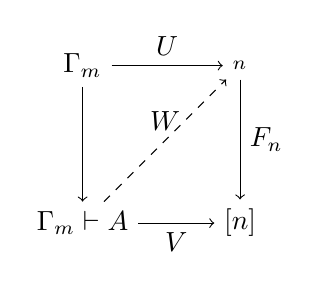
\begin{tikzpicture}
        \node (A) at (0,0) {$\gen{\Gamma_m}$};
        \node (X) at (2,0) {$\bS_n$};
        \node (B) at (0,-2) {$\gen{\Gamma_m\vdash A}$};
        \node (Y) at (2,-2) {$[n]$};
        \draw[->] (A) to (B);
        \draw[->] (A) to node[above]{$U$} (X);
        \draw[->] (X) to node[right]{$F_n$} (Y);
        \draw[->] (B) to node[below]{$V$} (Y);
        \draw[->, dashed] (B) to node[above]{$W$} (X);
    \end{tikzpicture}\end{matrix}\qquad
    \begin{matrix}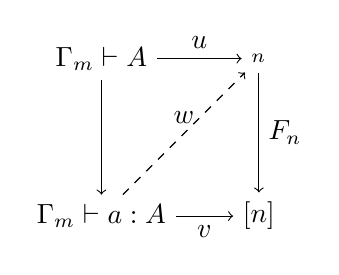
\begin{tikzpicture}
        \node (A) at (0,0) {$\gen{\Gamma_m\vdash A}$};
        \node (X) at (2,0) {$\bS_n$};
        \node (B) at (0,-2) {$\gen{\Gamma_m\vdash a:A}$};
        \node (Y) at (2,-2) {$[n]$};
        \draw[->] (A) to (B);
        \draw[->] (A) to node[above]{$u$} (X);
        \draw[->] (X) to node[right]{$F_n$} (Y);
        \draw[->] (B) to node[below]{$v$} (Y);
        \draw[->, dashed] (B) to node[above]{$w$} (X);
    \end{tikzpicture}\end{matrix}\]
    Since the maps $W$ and $w$ are defined by mapping out of a freely generated object, constructing the lift $W$ is equivalent to giving a type $X$ in context $U\Gamma_m$ for which $F_nX=VA$ (in context $V\Gamma_m$). Similarly, to define the lift $w$, we just need a term $x:uA$ in context $u\Gamma_m$ for which $F_nx=va$ (as terms of type $vA$ in context $v\Gamma_m$). These judgments are exactly what is given by proposition \ref{prop:liftJ}.
\end{proof}

\begin{prop}
    The cosimplicial object $\bS:\Delta\to\CxlCat_{\Id(,\Pi,\Sigma)}$ is Reedy cofibrant.
\end{prop}
\begin{proof}
    To prove this, we need to show that the natural map $L_n\bS\to\bS_n$ is a cofibration in $\CxlCat_{\Id(,\Pi,\Sigma)}$, where $L_n\bS$ is the $n$-th degree latching object of $\bS$. To do this, we will show that $\bS_n^{(n-1)}$ satisfies the universal property of the latching object. To see this, we note that the latching object is described as follows
    $$ L_n\bS=\colim_{\partial(\Delta_+\downarrow[n])}\bS_n=\colim\left(\coprod_{0\leq i<j\leq n}\bS_{n-2}\rightrightarrows\coprod_{0\leq i\leq n}\bS_{n-1}\right), $$
    %ellipses between the arrows?
    where the maps on the right are induced by the face inclusions, $\bS(d_i)\colon\bS_{n-2,i<j}\to\bS_{n-1,i}$ and $\bS(d_j)\colon\bS_{n-2,i<j}\to\bS_{n-1,j}$.

    To see that $\bS_n^{(n-1)}$ is the coequalizer of these maps, first we construct the map $\coprod\bS_{n-1}\to\bS_n^{(n-1)}$ by noting that the face inclusions $\bS(d_i):\bS_{n-1}\to\bS_n$ factor through $\bS_n^{(n-1)}$ as the remaining term in $\bS_n$ is not in the image of these maps. To see that this map coequalizes the maps in our colimit, we simply use the simplicial identities for face maps. Now, assume we have some theory $\T$ with a map $\coprod_{0\leq i\leq n}\bS_{n-1}\to\T$ that coequalizes the face inclusions. Since $\coprod_{0\leq i\leq n}\bS_{n-1}$ is a coproduct of freely generated theories, this amounts to a choice of $n$ closed types $C_i$ in $\T$ along with terms $x:C_i\vdash f_{ij}(x):C_j$ for all $0\leq i<j\leq n$, and identity terms $x:C_{\min(s)}\vdash c_s:\Id_{C_{\max(s)}}$ for all $s\subseteq [n]$, $\#s>2$, where the end points of the identity types are determined as they are when defining the terms $a_s$ in $S_{n}$. What this amounts to is essentially the choice of a boundary of an $n$-simplex in $\T$ with vertices given by closed types, edges given by functions, and higher cells given by identity types.

    To construct the map $\bS_{n}^{(n-1)}\to\T$, we note that the generators of $\bS_n^{(n-1)}$ are all of the generators of $\bS_n$ except the final $n$-cell (i.e. the term $a_{[n]}$), so we get the desired map by choosing exactly the same types and terms which were chosen by the previous map, making it clear that this map commutes with the rest of the diagram, and is unique by construction. This gives us that $L_n\bS=\bS_n^{(n-1)}$.

    Finally, to see that $\bS$ is Reedy cofibrant, we note that the map $\bS_n^{(n-1)}\to\bS_n$ is our model of the boundary inclusion, so $\bS_n$ only differs from $\bS_n^{(n-1)}$ by the addition of a single generating term (namely $a_{[n]}$), so this map is a cofibration in $\CxlCat_{\Id(,\Pi,\Sigma)}$ as desired.
\end{proof}

\begin{lem}
    Let $n\geq1$. The decomposition of $s_{n-1}(\gen{[n]})$ contains $\gen{\partial_i[n]}$ for all odd $i\in[n]$. Similarly for $t_{n-1}(\gen{[n]})$ and all even $i$.
\end{lem}
\begin{proof}
    First, we note that by definition, $s_{n-1}(\gen{[n]})_{n-1}^p=\{\partial_i[n]|i$ odd$\}$ and $s_{n-1}(\gen{[n]})_{m}^p=\emptyset$ for $p=0,1$ and $m>n-1$. This element $s_{n-1}(\gen{[n]})$ is then an $(n-1)$-cell (as it is in the image of $s_{n-1}$), but it is not equal to $\gen{z}$ for some $z\in s_{n-1}(\gen{[n]})_{n-1}^p$ (unless $n=1,2$, in which case the statement is trivial), as $s_{n-1}(\gen{[n]})_{n-1}^p=\{\partial_i[n]|i$ odd$\}$ will contain multiple elements ($\gen{z}_n^p=\{z\}$ for $p=0,1$ and $\#z=n$). This tells us that we can apply \ref{thm:decomp} repeatedly to get a decomposition of $s_{n-1}(\gen{[n]})$ into cells of the form $\gen{z_j}$ with $z_j\subseteq[n]$ and $\#z_j\leq n$, composed by $*_r$ for $r\leq n-2$. Since all compositions are taking place at levels $\leq n-2$, this means that $s_{n-1}(\gen{[n]})_{n-1}^p=\{\partial_i[n]|i$ odd$\}=\bigcup_i\gen{z_j}_{n-1}^p$ for all $\gen{z_j}$ in the decomposition. However, since each $\gen{z_j}$ is at most an $(n-1)$-cell, $\gen{z_j}_{n-1}^p$ is either empty for $\#z_j<n$ or equal to $z_j$ for $\#z_j=n$. This tells us that every $\partial_i[n]$ for $i$ odd must appear as one of the $z_j$ in the decomposition. The proof for $t_{n-1}(\gen{[n]})$ follows analogously.
\end{proof}

Note: $\gen{\partial_i[n]}$ ($0<i<n$) cannot be 0-composed with any element of the form $\gen{z}$ with $z\subseteq[n],\#z\geq2$ as that would require $s_0\gen{z}=\{n\}$ or $t_0\gen{z}=\{0\}$ which is not possible as $0\leq s_0\gen{z}=\{\min(z)\}<\{\max(z)\}=t_0\gen{z}\leq n$. % Probably just include this in the relavent proof

\begin{thm}
    The functor $N$ is valued in quasicategories.
\end{thm}
\begin{proof}
    
\end{proof}

\newpage

$$ \gen{[4]}=\begin{pmatrix}
        \{\{4\}\}, & \{\{0,1\},\{1,2\},\{2,3\},\{3,4\}\}, & \{\{0,1,2\},\{0,2,3\},\{0,3,4\}\}, & \{\{0,2,3,4\},\{0,1,2,4\}\}, & \{[4]\}, & \emptyset, & \dots\\
        \{\{0\}\}, & \{\{0,4\}\}, & \{\{0,1,4\},\{1,2,4\},\{2,3,4\}\}, & \{\{1,2,3,4\},\{0,1,3,4\},\{0,1,2,3\}\}, & \{[4]\}, & \emptyset, & \dots\\
    \end{pmatrix}. $$

\begin{align*}
    s_3\gen{01234}&=\gen{234}*_0\gen{12}*_0\gen{01}*_1\gen{0124}*_2\gen{34}*_0\gen{23}*_0\gen{012}*_1\gen{0234}\\
    t_3\gen{01234}&=\gen{1234}*_0\gen{01}*_1\gen{014}*_2\gen{34}*_0\gen{123}*\gen{01}*_1\gen{0134}*_0\gen{34?}*_0\gen{0123}*_1\gen{034}\\
\end{align*}
\begin{align*}
    a_{234}\circ_0a_{12}\circ_0a_{01}\circ_1a_{0124}:\Id_{A_4}^2(&a_{04},a_{34}\circ_0a_{23}\circ_0a_{12}\circ_0a_{01}:\\
    &a_{234}\circ_0a_{12}\circ_0a_{01}\circ_1a_{24}\circ_0a_{012}\circ_1a_{024},a_{234}\circ_0a_{12}\circ_0a_{01}\circ_1a_{124}\circ_0a_{01}\circ_1a_{014})\\
    a_{34}\circ_0a_{23}\circ_0a_{012}\circ_1a_{0234}:\Id_{A_4}^2(&a_{04},a_{34}\circ_0a_{23}\circ_0a_{12}\circ_0a_{01};\\
    &a_{34}\circ_0a_{23}\circ_0a_{012}\circ_1a_{34}\circ_0a_{023}\circ_1a_{034}, a_{34}\circ_0a_{23}\circ_0a_{012}\circ_1a_{234}\circ_0a_{02}\circ_1a_{024})
\end{align*}
In order to $2$-compose these, we need a path from
$$ a_{234}\circ_0a_{12}\circ_0a_{01}\circ_1a_{24}\circ_0a_{012}\circ_1a_{024}:=a_{234}(a_{12}(a_{01}(x)))*\ap_{a_{24}}(a_{012}(x))*a_{024}(x) $$
to
$$ a_{34}\circ_0a_{23}\circ_0a_{012}\circ_1a_{234}\circ_0a_{02}\circ_1a_{024}:=\ap_{a_{34}\circ a_{23}}(a_{012}(x))*a_{234}(a_{02}(x))*a_{024}(x). $$
Apply path induction to $a_{234}$ and $a_{012}$. Does this require lower cells to be in the context of higher cells that use them? ex. $x:A_0\vdash a_{012}(x):\Id_{A_2}(a_{02}(x),a_{12}(a_{01}(x)))$ vs. $x:A_0,a_{01}(x):A_1,a_{12}(x),a_{01}(x):A_2\vdash a_{012}(x):\Id_{A_2}(a_{02}(x),a_{12}(a_{01}(x)))$.

For target:
\begin{align*}
    a_{1234}\circ_0a_{01}\circ_1a_{014}:\Id_{A_4}^2(&a_{04},a_{34}\circ_0a_{23}\circ_0a_{12}\circ_0a_{01};\\
    &a_{34}\circ_0a_{123}\circ_1a_{134}\circ_0a_{01}\circ_1a_{014},a_{234}\circ_0a_{12}\circ_1a_{124}\circ_0a_{01}\circ_1a_{014})\\
    a_{34}\circ_0a_{123}\circ_0a_{01}\circ_1a_{0134}:\Id_{A_4}^2(&a_{04},a_{34}\circ_0a_{23}\circ_0a_{12}\circ_0a_{01};\\
    &a_{34}\circ_0a_{123}\circ_0a_{01}\circ_1a_{34}\circ_0a_{013}\circ_1a_{034},a_{34}\circ_0a_{123}\circ_0a_{01}\circ_1a_{134}\circ_0a_{01}\circ_1a_{014})\\
    a_{34}\circ_0a_{0123}\circ_1a_{034}:\Id_{A_4}^2(&a_{04},a_{34}\circ_0a_{23}\circ_0a_{12}\circ_0a_{01};\\
    &a_{34}\circ_0a_{23}\circ_0a_{012}\circ_1a_{023}\circ_1a_{034},a_{34}\circ_0a_{123}\circ_0a_{01}\circ_1a_{013}\circ_1a_{034})\\
\end{align*}
Now need paths between $a_{34}\circ_0(a_{123}\circ_0a_{01}\circ_1a_{013})\circ_1a_{034}:=(\ap_{a_{34}}(a_{123}(a_{01}(x))*a_{013}(x)))*a_{034}(x)$ and $(a_{34}\circ_0a_{123}\circ_0a_{01})\circ_1(a_{34}\circ_0a_{013}\circ_1a_{034}):=(\ap_{a_{34}}(a_{123}(a_{01}(x))))*(\ap_{a_{34}}(a_{013}(x))*a_{034}(x))$ (given by $\ap$ distributing over comp. and associativity), and \newline
$(a_{34}\circ_0a_{123}\circ_0a_{01})\circ_1(a_{134}\circ_0a_{01}\circ_1a_{014}):=(\ap_{a_{34}}(a_{123}(a_{01}(x)))*(a_{134}(a_{01}(x))*a_{014}(x))$ and \newline
$((a_{34}\circ_0a_{123}\circ_1a_{134})\circ_0a_{01})\circ_1a_{014}:=(\ap_{a_{34}}(a_{123})*a_{134})(a_{01}(x))*a_{014}(x)$ (given by associativity and since $p(x)*q(x):=(p*q)(x)$).

Assuming we can do these compositions, we get
$$ |s_3\gen01234|:\Id_{A_4}^2(-,-;(a_{34}\circ_0a_{23}\circ_0a_{01})\circ_1(a_{34}\circ_0a_{023}\circ_1a_{034}),(a_{234}\circ_0a_{12}\circ_0a_{01})\circ_1(a_{124}\circ_0a_{01}\circ_1a_{014})), $$
$$ |t_3\gen{01234}|:\Id_{A_4}^2(-,-;(a_{34}\circ_0(a_{23}\circ_0a_{012}\circ_1a_{023}))\circ_1a_{034},((a_{234}\circ_0a_{12}\circ_1a_{124})\circ_0a_{01})\circ_1a_{014}). $$
Targets are definitionally equal (distributivity of dependency), sources are $\ap_{a_{34}\circ a_{23}}(a_{012}(x))*(\ap_{a_{34}}(a_{023}(x))*a_{034}(x))$ and $\ap_{a_{34}}(\ap_{a_{23}}(a_{012}(x))*a_{023}(x))*a_{034}(x)$.

Can solve this by inserting the relevant paths into the terms (this doesn't seem like a good solution). Or, we can transport along the relevant paths, so we can strictly compose and form the correct type for $a_{01234}$ (this still seems like it's not particularly scalable for higher dimensions). Redefining composable pairs to be less strict may help, but it may not be good enough for higher dimensions.


% \newpage
% \section{Alternate Definitions}

% \begin{defn}
%     Let
%     $$ \Gamma(\T,S)_0:=S, $$
%     $$ \Gamma(\T,S)_1=\left\{(A_0,A_1;\gamma)\ |\ A_i\in\Gamma(\T,S)_0\text{ and }\vdash\gamma:\Id^0_{A_0\to A_1}\right\}, $$
%     with $s_1,t_1$ being the first and second projections respectively. From here, we define the remaining levels inductively. For $n>1$, we define
%     $$ \Gamma(\T,S)_{n+1}:=\left\{(A_0,A_1;\vec{\alpha};\beta_0,\beta_1;\gamma)\ |\ (A_0,A_1;\vec{\alpha};\beta_i)\in\Gamma(\T,S)_n\text{ and }\vdash\gamma:\Id_{A_0\to A_1}^{n}(\vec{\alpha};\beta_0,\beta_1)\right\}, $$
%     with $s_{n+1},t_{n+1}$ given by $(A_0,A_1;\vec{\alpha};\beta_0,\beta_1;\gamma)\mapsto(A_0,A_1;\vec{\alpha};\beta_i)$ with $i=0,1$ respectively. Reflexivity at level 0 is given by the map $i_0:\Gamma(\T,S)_0\to\Gamma(\T,S)_1$ which sends $A$ to  $(A,A;\lambda x.x\colon 
%     A\to A)$. Above level 0, reflexivity is given by the maps $i_n:\Gamma(\T,S)_n\to\Gamma(\T,S)_{n+1}$ which sends $(\vec{\alpha};\beta)$ to $(\vec{\alpha};\beta,\beta;\refl_\beta)$. The relevant identities are easily verified.
% \end{defn}

% \begin{defn}
%     For $n=1$, we define
%     $$ (A_0,A_1;\gamma)\circ_0(A_0',A_1';\gamma'):=(A_0',A_1;\gamma\circ\gamma'), $$
%     noting that $A_0=A_1'$ because our cells are 0-composable. Now assuming we can $m$-compose $n$ cells for all $m<n$, we define $m$-composition of $(n+1)$-cells,
%     $$ (A_0,A_1;\vec{\alpha};\beta_0,\beta_1;\gamma)\circ_m(A'_0,A'_1;\vec{\alpha}';\beta_0',\beta_1';\gamma') $$
%     with two cases. First, if $m=n$, then our inductive hypothesis cannot help us, so we instead just apply path concatenation (which path concatenation?), which applies as $(A_0,A_1;\vec{\alpha};\beta_0,\beta_1;\gamma)$ and $(A'_0,A'_1;\vec{\alpha}';\beta_0',\beta_1';\gamma')$ are $n$-composable, so we get
%     $$ (A_0,A_1;\vec{\alpha};\beta_0,\beta_1;\gamma)\circ_m(A'_0,A'_1;\vec{\alpha}';\beta_0',\beta_1';\gamma'):=(A_0,A_1;\vec{\alpha};\beta_0',\beta_1;\gamma*\gamma'). $$
%     If $m<n$, then we apply path induction to both $\gamma$ and $\gamma'$ to reduce the problem to
%     \begin{align*}
%         (A_0,A_1;\vec{\alpha};\beta_0,\beta_0;\refl_{\beta_0})\circ_m(A'_0,A'_1;\vec{\alpha}';\beta_0',\beta_0';\refl_{\beta_0'})&=i_{n+1}(A_0,A_1;\vec{\alpha};\beta_0)\circ_mi_{n+1}(A'_0,A'_1;\vec{\alpha}';\beta_0')\\
%         &:=i_{n+1}\left((A_0,A_1;\vec{\alpha};\beta_0)\circ_m(A'_0,A'_1;\vec{\alpha}';\beta_0')\right).
%     \end{align*}
% \end{defn}

% \begin{defn}
%     Given $n\in\N$, we define the type theory $\bS_n^{(i+1)}$ to be the type theory freely generated by the generators of $\bS_n^{(i)}$ along with closed terms
%     $$ a_z:\Id^{i-1}_{A_{\min(z)}\to A_{\max(z)}}\left(|s_j(\gen{z})|_j,|t_j(\gen{z})|_j\right)\qquad(1\leq j\leq i), $$
%     for all $z\subseteq[n]$ such that $\#z=i+1$.
% \end{defn}

% Note that by $|s_j(\gen{z})|_j,|t_j(\gen{z})|_j$, we really mean the final projection of this element which is a term of the correct type as opposed to an element of $\Gamma(\bS_n^{(j)})$.

% \begin{defn}
%     Given $n\in\N$, we define a function
%     $$ |-|_{i+1}\colon\mathcal{O}_{n,i+1}\to\bigsqcup_{m\in\N}\Gamma\left(\bS_n^{(i+1)}\right)_m $$
%     by sending $b\in\mathcal{O}_{n,i+1}$ to $|b|_i$ if $b\in\mathcal{O}_{n,i}$, or $\alpha_{b_1}=\left(|s_j(\gen{s})|_j,|t_j(\gen{s})|_j,a_{b_1}\right)$ if $b=\gen{b_1}$ for some $b_1\subseteq[n]$. Otherwise, we apply Cor. 3.14 to get $b=b_1*_{k}b_2$ and we send this element to $|b_1|_{i+1}\circ_{k}|b_2|_{i+1}$.
% \end{defn}


\bibliographystyle{plain}
\bibliography{refs}

\end{document}